%%%%%%%%%%%%%%%%%%%%%%%%%%%%%%%%%%%%%%%%%
% Beamer Presentation
% LaTeX Template
	% Version 1.0 (10/11/12)
%
% This template has been downloaded from:
% http://www.LaTeXTemplates.com
%
% License:
% CC BY-NC-SA 3.0 (http://creativecommons.org/licenses/by-nc-sa/3.0/)
%
%%%%%%%%%%%%%%%%%%%%%%%%%%%%%%%%%%%%%%%%%

%----------------------------------------------------------------------------------------
%	PACKAGES AND THEMES
%----------------------------------------------------------------------------------------

\documentclass[10pt, xcolor=x11names]{beamer}

\mode<presentation> {


% The Beamer class comes with a number of default slide themes
% which change the colors and layouts of slides. Below this is a list
% of all the themes, uncomment each in turn to see what they look like.

%\usetheme{default}
%\usetheme{AnnArbor}
%\usetheme{Antibes}
%\usetheme{Bergen}
%\usetheme{Berkeley}
%\usetheme{Berlin}
%\usetheme{Boadilla}
%\usetheme{CambridgeUS}
\usetheme{Copenhagen} %boa hein?
%\usetheme{Darmstadt}
%\usetheme{Dresden}
%\usetheme{Frankfurt} %bonzin tb
%\usetheme{Goettingen}
%\usetheme{Hannover}
%\usetheme{Ilmenau}
%\usetheme{JuanLesPins} % mais ou menos tambem
%\usetheme{Luebeck}
%\usetheme{Madrid} %azulsinho default
%\usetheme{Malmoe}
%\usetheme{Marburg}
%\usetheme{Montpellier}
%\usetheme{PaloAlto}
%\usetheme{Pittsburgh}
%\usetheme{Rochester}
%\usetheme{Singapore}
%\usetheme{Szeged}
%\usetheme{Warsaw}

% As well as themes, the Beamer class has a number of color themes
% for any slide theme. Uncomment each of these in turn to see how it
% changes the colors of your current slide theme.

%\usecolortheme{albatross}
%\usecolortheme{beaver}
%\usecolortheme{beetle}
%\usecolortheme{crane}
%\usecolortheme{dolphin} %gostei
%\usecolortheme{dove}
%\usecolortheme{fly}
%\usecolortheme{lily}
%\usecolortheme{orchid}
%\usecolortheme{rose}
%\usecolortheme{seagull}
%\usecolortheme{seahorse} %gostei tb
%\usecolortheme{whale}
%\usecolortheme{wolverine}

\setbeamertemplate{footline} % To remove the footer line in all slides uncomment this line
%\setbeamertemplate{footline}[page number]{} % To replace the footer line in all slides with a simple slide count uncomment this line

%\setbeamertemplate{navigation symbols}{} % To remove the navigation symbols from the bottom of all slides uncomment this line


%\setbeamercovered{transparent} % To set the itens transparents
\setbeamercovered{transparent=3} %(default is 15% opaqueness)
%\setbeamercovered{invisible}	% To set the itens ivisibles is default settings
\usefonttheme[onlymath]{serif}
%\setbeamertemplate{headline}[default]
%\setbeamertemplate{navigation symbols}{}
\mode<beamer>{\setbeamertemplate{blocks}[rounded][shadow=true]}
\setbeamercolor{block body example}{fg=blue, bg=black!20}
}

\usepackage{graphicx} % Allows including images
\usepackage{xcolor}
\usepackage{booktabs} % Allows the use of \toprule, \midrule and \bottomrule in tables
\usepackage[brazil]{babel}   
\usepackage[utf8]{inputenc}  
\usepackage{caption}  %Allows including capitons on images
%\usepackage{subcaption} %allow including multiples figures side to side
\usepackage{ragged2e} %allows justify text
\usepackage{url}
\usepackage{amssymb}

\usepackage{lipsum}
\newcommand\Fontvi{\fontsize{8}{7.2}\selectfont}

%----------------------------------------------------------------------------------------
%	TITLE PAGE
%----------------------------------------------------------------------------------------

\title[Sockets - Múltiplas Conexões]{Sockets - Múltiplas Conexões \\ Usando: THREADS e SELECT} % The short title appears at the bottom of every slide, the full title is only on the title page
%\subtitle[short version]{A subtitle}
\author[Bruno P. Santos]{Bruno Pereira}% Your name
\institute[ UFMG ]% Your institution as it will appear on the bottom of every slide, may be shorthand to save space
{
Universidade Federal de Minas Gerais \\ % Your institution for the title page
\medskip
\textit{bruno.ps@live.com} % Your email address
}
\date{\today} % Date, can be changed to a custom date

\begin{document}

\begin{frame}
\titlepage % Print the title page as the first slide
\end{frame}


\begin{frame}
\frametitle{Roteiro} % Table of contents slide, comment this block out to remove it
\tableofcontents % Throughout your presentation, if you choose to use \section{} and \subsection{} commands, these will automatically be printed on this slide as an overview of your presentation
\end{frame}

%----------------------------------------------------------------------------------------
%	PRESENTATION SLIDES
%----------------------------------------------------------------------------------------

%------------------------------------------------
\section{Introdução} % Sections can be created in order to organize your presentation into discrete blocks, all sections and subsections are automatically printed in the table of contents as an overview of the talk
%------------------------------------------------

\begin{frame} \frametitle{Introdução}
	
	\begin{columns}
		\column{0.6\textwidth}
			\begin{block}{Relembrando}	
				\begin{itemize}
					\item<1-> Até o momento...
					\begin{itemize}
						\item Sabemos trocar dados entre:
							\begin{itemize}
							 	\item \textbf{UM} Cliente e \textbf{UM} Servidor
							\end{itemize} 
						\item Tratar conexões IPv*
						\item Transporte: STREAM vs DGRAM
					\end{itemize}
					\item<2->  Agora queremos...
					\begin{itemize}
						\item Manipular conexões simultaneamente!
					\end{itemize}
					\item<3->  Como fazer ?
					\begin{itemize}
						\item \textcolor{red}{\textbf{Threads}}
						\item \textcolor{red}{\textbf{Select}}
						\item Processos
					\end{itemize}
				\end{itemize}
			\end{block}
		\column{0.5\textwidth}
			\begin{figure}
			\centering
				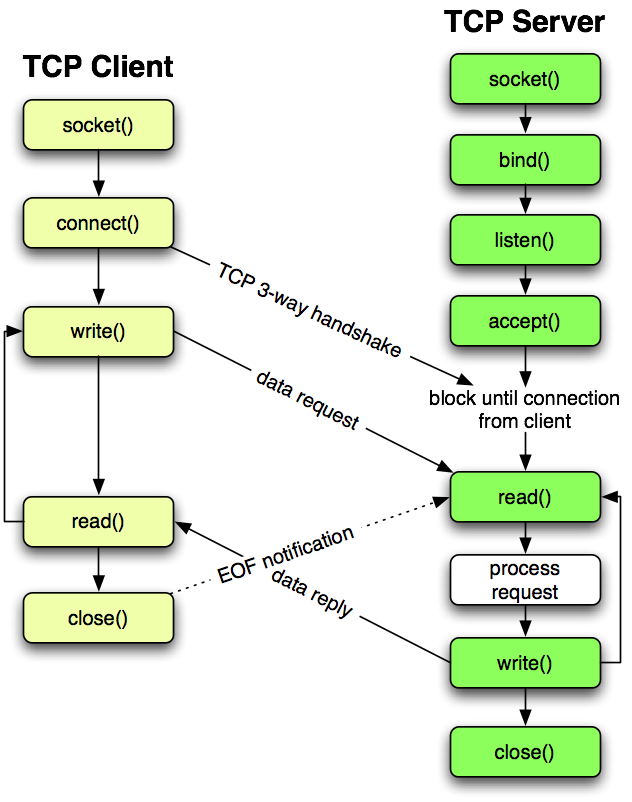
\includegraphics[width=1\linewidth]{img/tcplab}<1>
			\end{figure}
			\begin{figure}
			\centering
				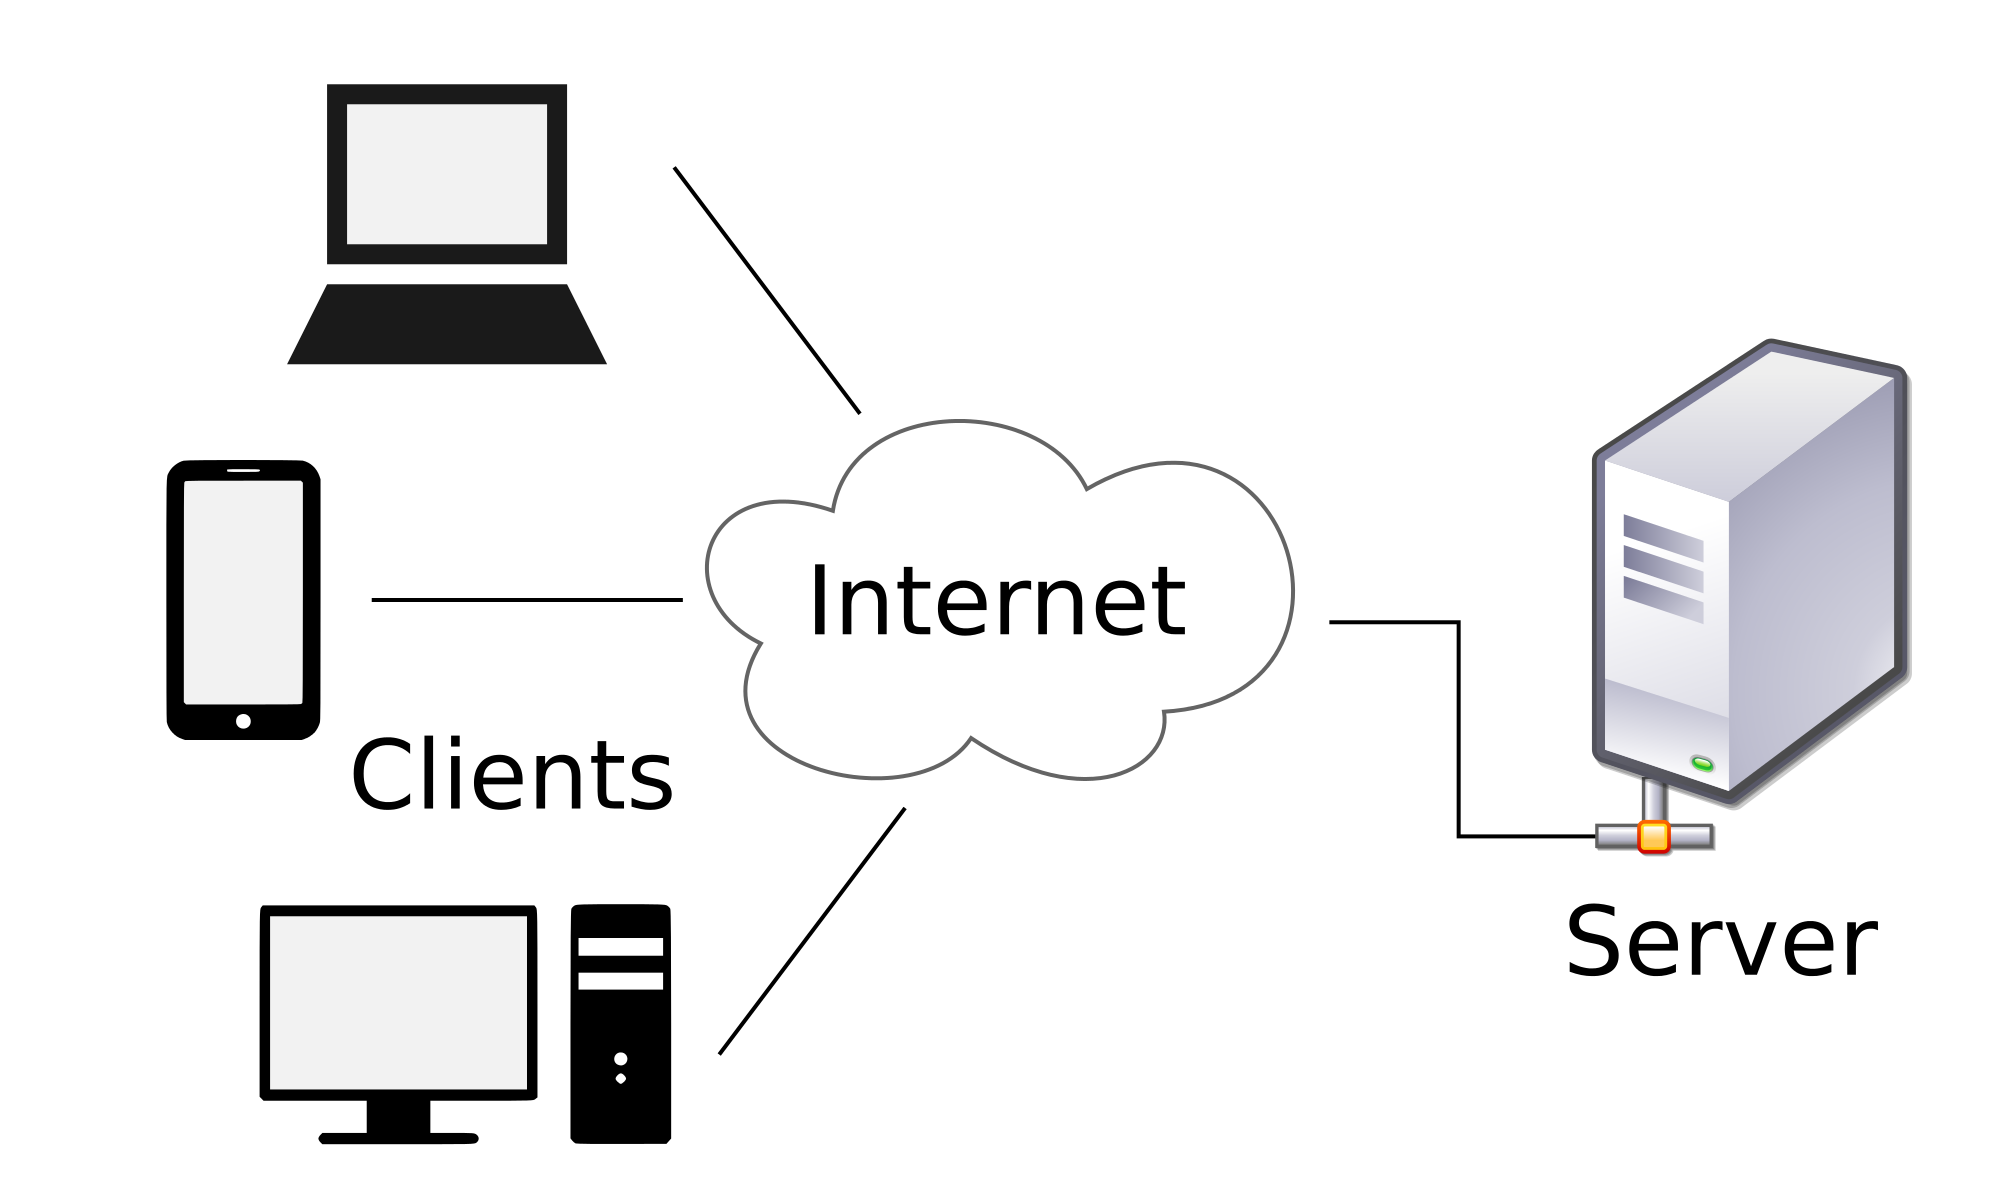
\includegraphics[width=1\linewidth]{img/multiple-clients}<2->
			\end{figure}
	\end{columns}

\end{frame}

\begin{frame}
	\begin{block}{Objetivos}
		\begin{itemize}
			\item Ao final dessa aula você será capaz de:
			\begin{itemize}
				\item Entender o uso de threads
				\item Entender o uso do \textit{Select}
			\end{itemize}
			\item Criar um programa \textbf{SERVIDOR} que aceita conexão de vários clientes
			\begin{itemize}
				\item Usando \textcolor<2->{red}{\textit{Threads}}
				\item Usando \textit{Select}
			\end{itemize}
		\end{itemize}
		\begin{itemize}
			\item<2-> Vamos criar um \textbf{SERVIDOR} que cria uma \textbf{THREAD} para cada cliente
			\begin{itemize}
				\item Cada threads cuidará da lógica/execução de cada cliente individualmente
			\end{itemize}
		\end{itemize}
	\end{block}
\end{frame}

%------------------------------------------------
\subsection{Entendendo Threads} % A subsection can be created just before a set of slides with a common theme to further break down your presentation into chunks


\begin{frame} %\frametitle{Entendendo os Sockets}
	\begin{block}{O que é Thread?}
		\begin{itemize}
			\item<1-> Antes de definir threads vamos entender o que é um \textcolor<2->{red}{PROCESSO}.

			\item<4-> Em um processo existe uma thread (uma linha de execução)
		\end{itemize}
	\end{block}

	\begin{columns}<2-4>
		\column{0.5\textwidth}
			\begin{alertblock}{\textbf{PROCESSO}}<2-4>
				\begin{itemize}
					\item Um processo é uma instância de um programa que está em \textit{execução}
					\item Está em um dos seus 5 estados
					\item Possui vários atributos no seu \textit{Process Control Block}
 				\end{itemize}
			\end{alertblock}

		\column{0.5\textwidth}
			\begin{figure}
			\centering
				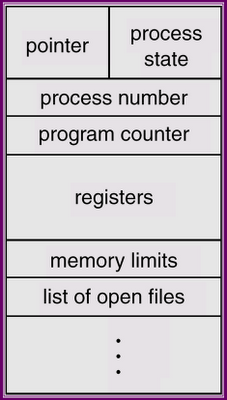
\includegraphics[width=.6\linewidth]{img/pcb.png}<4>
			\end{figure}
			\begin{figure}
			\centering
				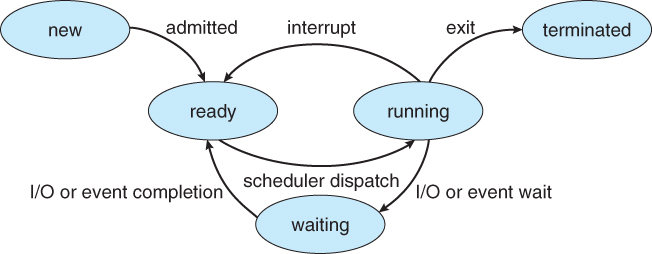
\includegraphics[width=1.1\linewidth]{img/process_states.png}<3>
			\end{figure}
			
	\end{columns}
	
\end{frame}
%------------------------------------------------

\begin{frame} %\frametitle{Entendendo os Sockets}
	\begin{block}{O que é Thread?}
		\begin{itemize}
			\item Antes de definir threads vamos entender o que é um \textcolor{red}{PROCESSO}.

			\item Em um processo existe uma thread (uma linha de execução)
		\end{itemize}
	\end{block}

	\begin{alertblock}{Thread}<2->
		\textbf{Thread (linha de execução) é o menor fluxo sequencial de execução dentro de um programa, o qual pode ser gerenciado por um escalonador.}
	\end{alertblock}
	
\end{frame}
%------------------------------------------------

\begin{frame}
	\begin{alertblock}{Thread}
		\textbf{Thread (linha de execução) é o menor fluxo sequencial de execução dentro de um programa, o qual pode ser gerenciado por um escalonador.}
	\end{alertblock}

	\begin{figure}
	\centering
		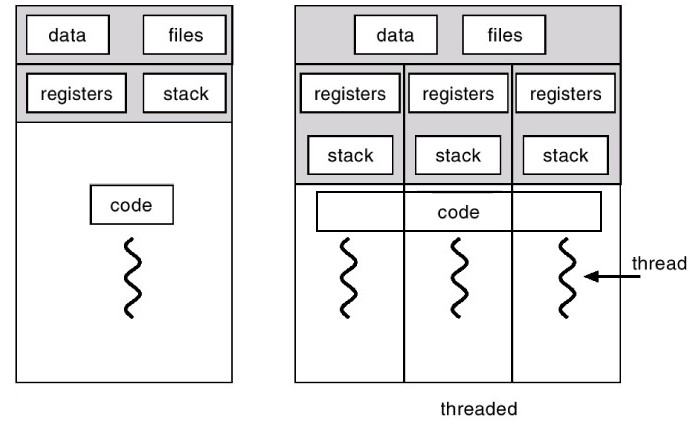
\includegraphics[width=1\linewidth]{img/Thread-1}
	\end{figure}

\end{frame}

%------------------------------------------------

\begin{frame}
	\begin{alertblock}{Thread}
		\textbf{Thread (linha de execução) é o menor fluxo sequencial de execução dentro de um programa, o qual pode ser gerenciado por um escalonador.}
	\end{alertblock}
	\begin{columns}
		\column{0.5\textwidth}
		\begin{figure}
		\centering
			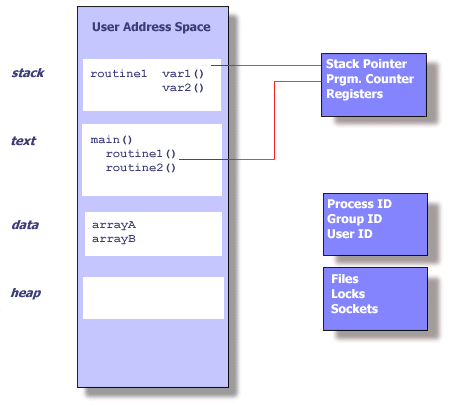
\includegraphics[width=1\linewidth]{img/process}<1->
		\end{figure}

		\column{0.5\textwidth}
		\begin{figure}
		\centering
			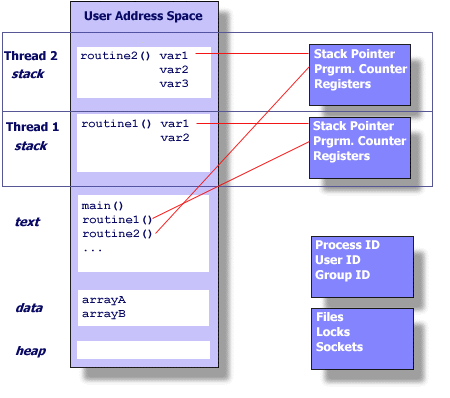
\includegraphics[width=1.\linewidth]{img/thread.png}<2->
		\end{figure}
	\end{columns}

\end{frame}

%------------------------------------------------

\begin{frame}
	\begin{block}{Diferenças entre Threads e Processos}
		\begin{figure}
		\centering
			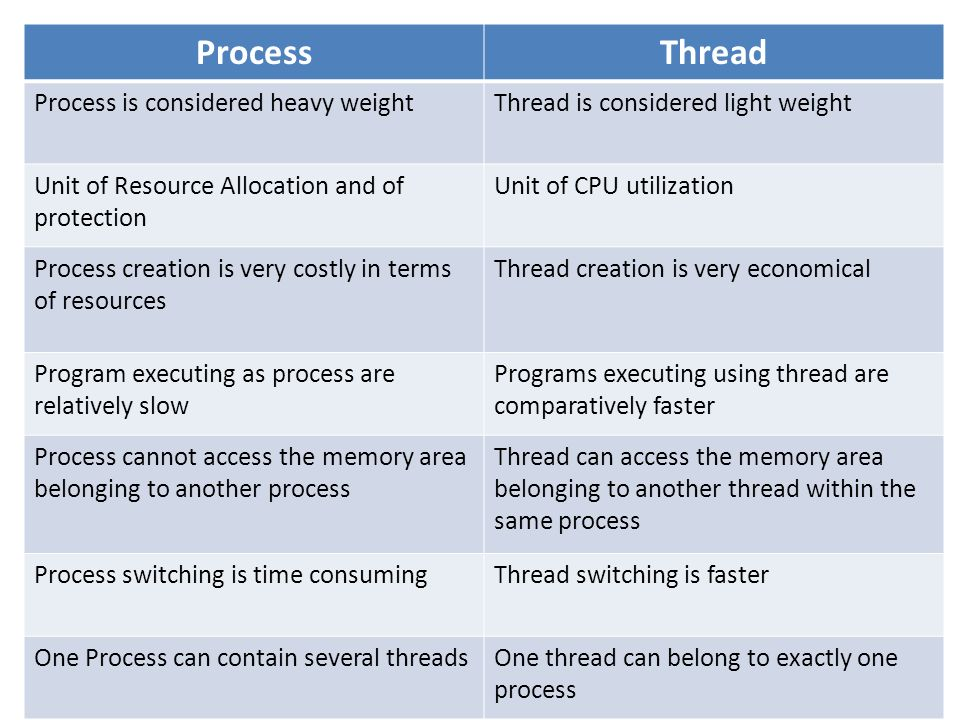
\includegraphics[width=.8\linewidth]{img/diff-proc-thre.jpg}
		\end{figure}
	\end{block}
\end{frame}

%------------------------------------------------
\subsection{O que são Pthreads?} % A subsection can be created just before a set of slides with a common theme to further break down your presentation into chunks

\begin{frame} \frametitle{Como vamos usar Threads?}
	\begin{block}{Através da biblioteca Pthreads -- Visão Geral}
		\begin{itemize}[<+->]
			\item Historicamente grandes empresas de HW tinham suas próprias implementações de threads
			\item Isto gerou:
				\begin{itemize}
					\item Dificuldades de desenvolvidmento e portabilidade
				\end{itemize}
			\item Então foi necessário criar uma padronização
				\begin{itemize}
					\item Para sistemas UNIX (Solares, Linux) foi especificado o padrão IEEE POSIX 1003.1c standard (1995)\footnote{Existe implementações para Windows}
					\item Implementações que usam esse padrão são referenciadas como POSIX threads (Pthreads)
				\end{itemize}
		\end{itemize}
	\end{block}

	\begin{block}{Links Úteis}<7->
		\begin{itemize}
			\item \url{https://computing.llnl.gov/tutorials/pthreads/}
			\item \url{http://www.opengroup.org/austin/papers/posix_faq.html}
			
		\end{itemize}
	\end{block}
\end{frame}

%------------------------------------------------
\section{Usando PTHREADS} 

\begin{frame}
	\begin{block}{Pthread API}
		\begin{itemize}
			\item<1-> As subrotinas da API Pthreads podem ser agrupadas em 4 grandes grupos:
				\begin{enumerate}
					\item<1-> \textcolor<5->{red}{\textbf{Gerenciamento de Threads:} rotinas para criar, desanexar, agrupar. Além de funções para consultar atributos das threads}	

					\item<2-> \textcolor<5->{gray}{\textbf{Mutexes:} rotinas para criar sincronizações para áreas críticas. Existem funções para criar, destruir, travar e destravar mutexes}

					\item<3-> \textcolor<5->{gray}{\textbf{Condition variables:} rotinas para lidar com a comunicação entre threads que compartilham um mutex}

					\item<4-> \textcolor<5->{gray}{\textbf{Sincronização:} rotinas que gerenciam leituras/escritas em seções críticas}
				\end{enumerate}
			
		\end{itemize}
	\end{block}
\end{frame}

%------------------------------------------------
\subsection{Pthreads -- Primitivas básicas} % A subsection can be created just before a set of slides with a common theme to further break down your presentation into chunks

\begin{frame}
	
int \textcolor{red}{pthread\_create}(\textcolor{purple}{pthread\_t * thread}, \textcolor{blue}{pthread\_attr\_t *attr},\\ \hspace{2.7cm} \textcolor{orange}{void * (*start\_routine)(void *)}, \textcolor[rgb]{.6,0,1}{void * arg});

	\begin{block}{Criar uma thread}
		\begin{itemize}[<+->]
			\item \textcolor{purple}{pthread\_t * thread}: identificador único para uma nova thread (retornado pela subrotina)
			\item \textcolor{blue}{pthread\_attr\_t *attr}: estrutura para definir valores dos atributos da thread
				\begin{itemize}
					\item Política de escalonamento
					\item Tamanho da pilha...
				\end{itemize}
			\item \textcolor{orange}{void * (*start\_routine)(void *)}: uma FUNÇÃO EM C QUE A THREAD EXECUTARÁ
			\item \textcolor[rgb]{.6,0,1}{void * arg}\footnote{Esse argumento deve ser passado por referência. Atente-se para o cast para void}: arumento recebido por ``\textcolor{orange}{*start\_routine}". Use NULL para valores padrão.
		\end{itemize}
	\end{block}
\end{frame}

%------------------------------------------------

\begin{frame}
	
int \textcolor{red}{pthread\_create}(\textcolor{purple}{pthread\_t * thread}, \textcolor{blue}{pthread\_attr\_t *attr},\\ \hspace{2.7cm} \textcolor{orange}{void * (*start\_routine)(void *)}, \textcolor[rgb]{.6,0,1}{void * arg});

	\begin{block}{Retorno}
		\begin{itemize}
			\item 0, se tudo Ok!
			\item Valor indicando um dos possíveis erros.
		\end{itemize}
	\end{block}

\end{frame}

%------------------------------------------------

\begin{frame}
	\begin{alertblock}{Question time!}

		\begin{itemize}
			\item Q: Dado que a thread foi criada como você saberá:
				\begin{itemize}
					\item Quando a thread será escalonada para executar pelo SO?
					\item Qual processaor/núcleo ela irá executar?	
				\end{itemize}
		\end{itemize}
	\end{alertblock}

	\begin{columns}	
		\column{0.7\textwidth}
			\begin{block}{Resposta}<2->
				Programas robustos não depedem de uma ordem específica para executar as threads. \\
				O SO irá decidir \textbf{quando e onde} executar as treads. \\
				\textcolor{red}{NÃO PRECISAMOS TRATAR ISSO!}				
			\end{block}

		\column{0.3\textwidth}
			\begin{figure}
				
\includegraphics[width=.55\linewidth]{img/question-meme.jpg}<1>
			\end{figure}	
			\begin{figure}
				
\includegraphics[width=.55\linewidth]{img/question-answer.jpg}<2->
			\end{figure}
 			
	\end{columns}
\end{frame}
%------------------------------------------------

\begin{frame}

void \textcolor{red}{pthread\_exit}(\textcolor{purple}{void * retval});

	\begin{block}{Terminar a execução thread}
		\begin{itemize}
			\item \textcolor{purple}{void * retval}: valor de retorno da thread
				\begin{itemize}
					\item Uma thread por terminar por vários motivos:
						\begin{itemize}
							\item Retornam normalmente da sua função ``\textcolor{orange}{*start\_routine}"
							\item Fazendo uma chamada para a subrotina \textcolor{red}{pthread\_exit}
							\item Pode ser cancelada por outra thread via subrotina pthread\_cancel
							\item ...
						\end{itemize}
					
				\end{itemize}
		\end{itemize}
	\end{block}

	\begin{alertblock}{Dica}
		\begin{itemize}
			\item Se a thread mãe termina retornando da sua função principal, então suas filhas morrem.
			\item Se a thread mãe termina com pthread\_exit(), suas filhas não morrem.
		\end{itemize}
	\end{alertblock}

\end{frame}

%------------------------------------------------

\begin{frame}

void \textcolor{red}{pthread\_join}(\textcolor{purple}{pthread\_t * thread}, \textcolor{blue}{pthread\_attr\_t **status});

	\begin{block}{Terminar a execução thread}
		\begin{itemize}
			\item \textcolor{purple}{pthread\_t * thread}: indica a thread a ser aguardada
			\item \textcolor{blue}{pthread\_attr\_t **status}: valor de retorno da thread
		\end{itemize}
	\end{block}

	\begin{columns}
		\column{0.4\textwidth}
			\begin{alertblock}{Dica}
				Essa função faz com que a thread que a chamou espere até que a thread passada como parâmetro retorne
			\end{alertblock}

		

		\column{0.6\textwidth}
		\begin{flushright}
			\begin{figure}
				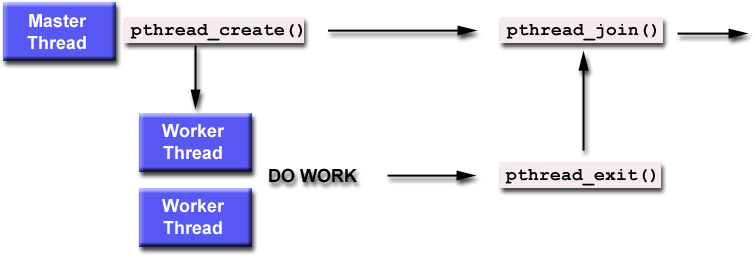
\includegraphics[width=1.1\linewidth]{img/joining.png}
			\end{figure}
		\end{flushright}	
		
	\end{columns}

	
\end{frame}


%------------------------------------------------
\subsection{1º Código com Threads}
%------------------------------------------------
\begin{frame}
	\begin{columns}
		\column{0.8\textwidth}
			\begin{figure}
				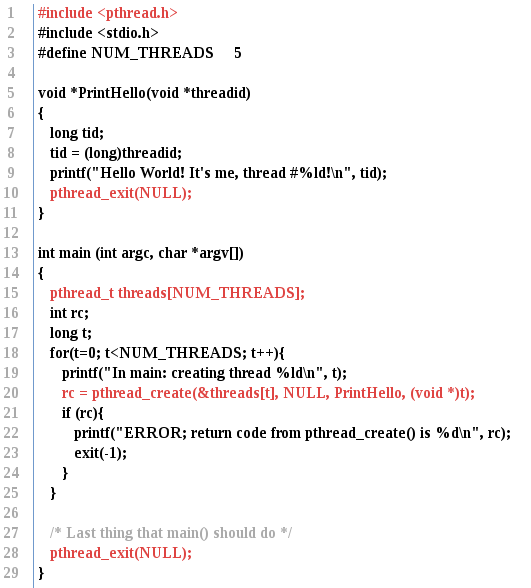
\includegraphics[width=.8\linewidth]{img/code-thread.png}
			\end{figure}
		

		\column{0.2\textwidth}
		\begin{flushright}
			\begin{figure}
				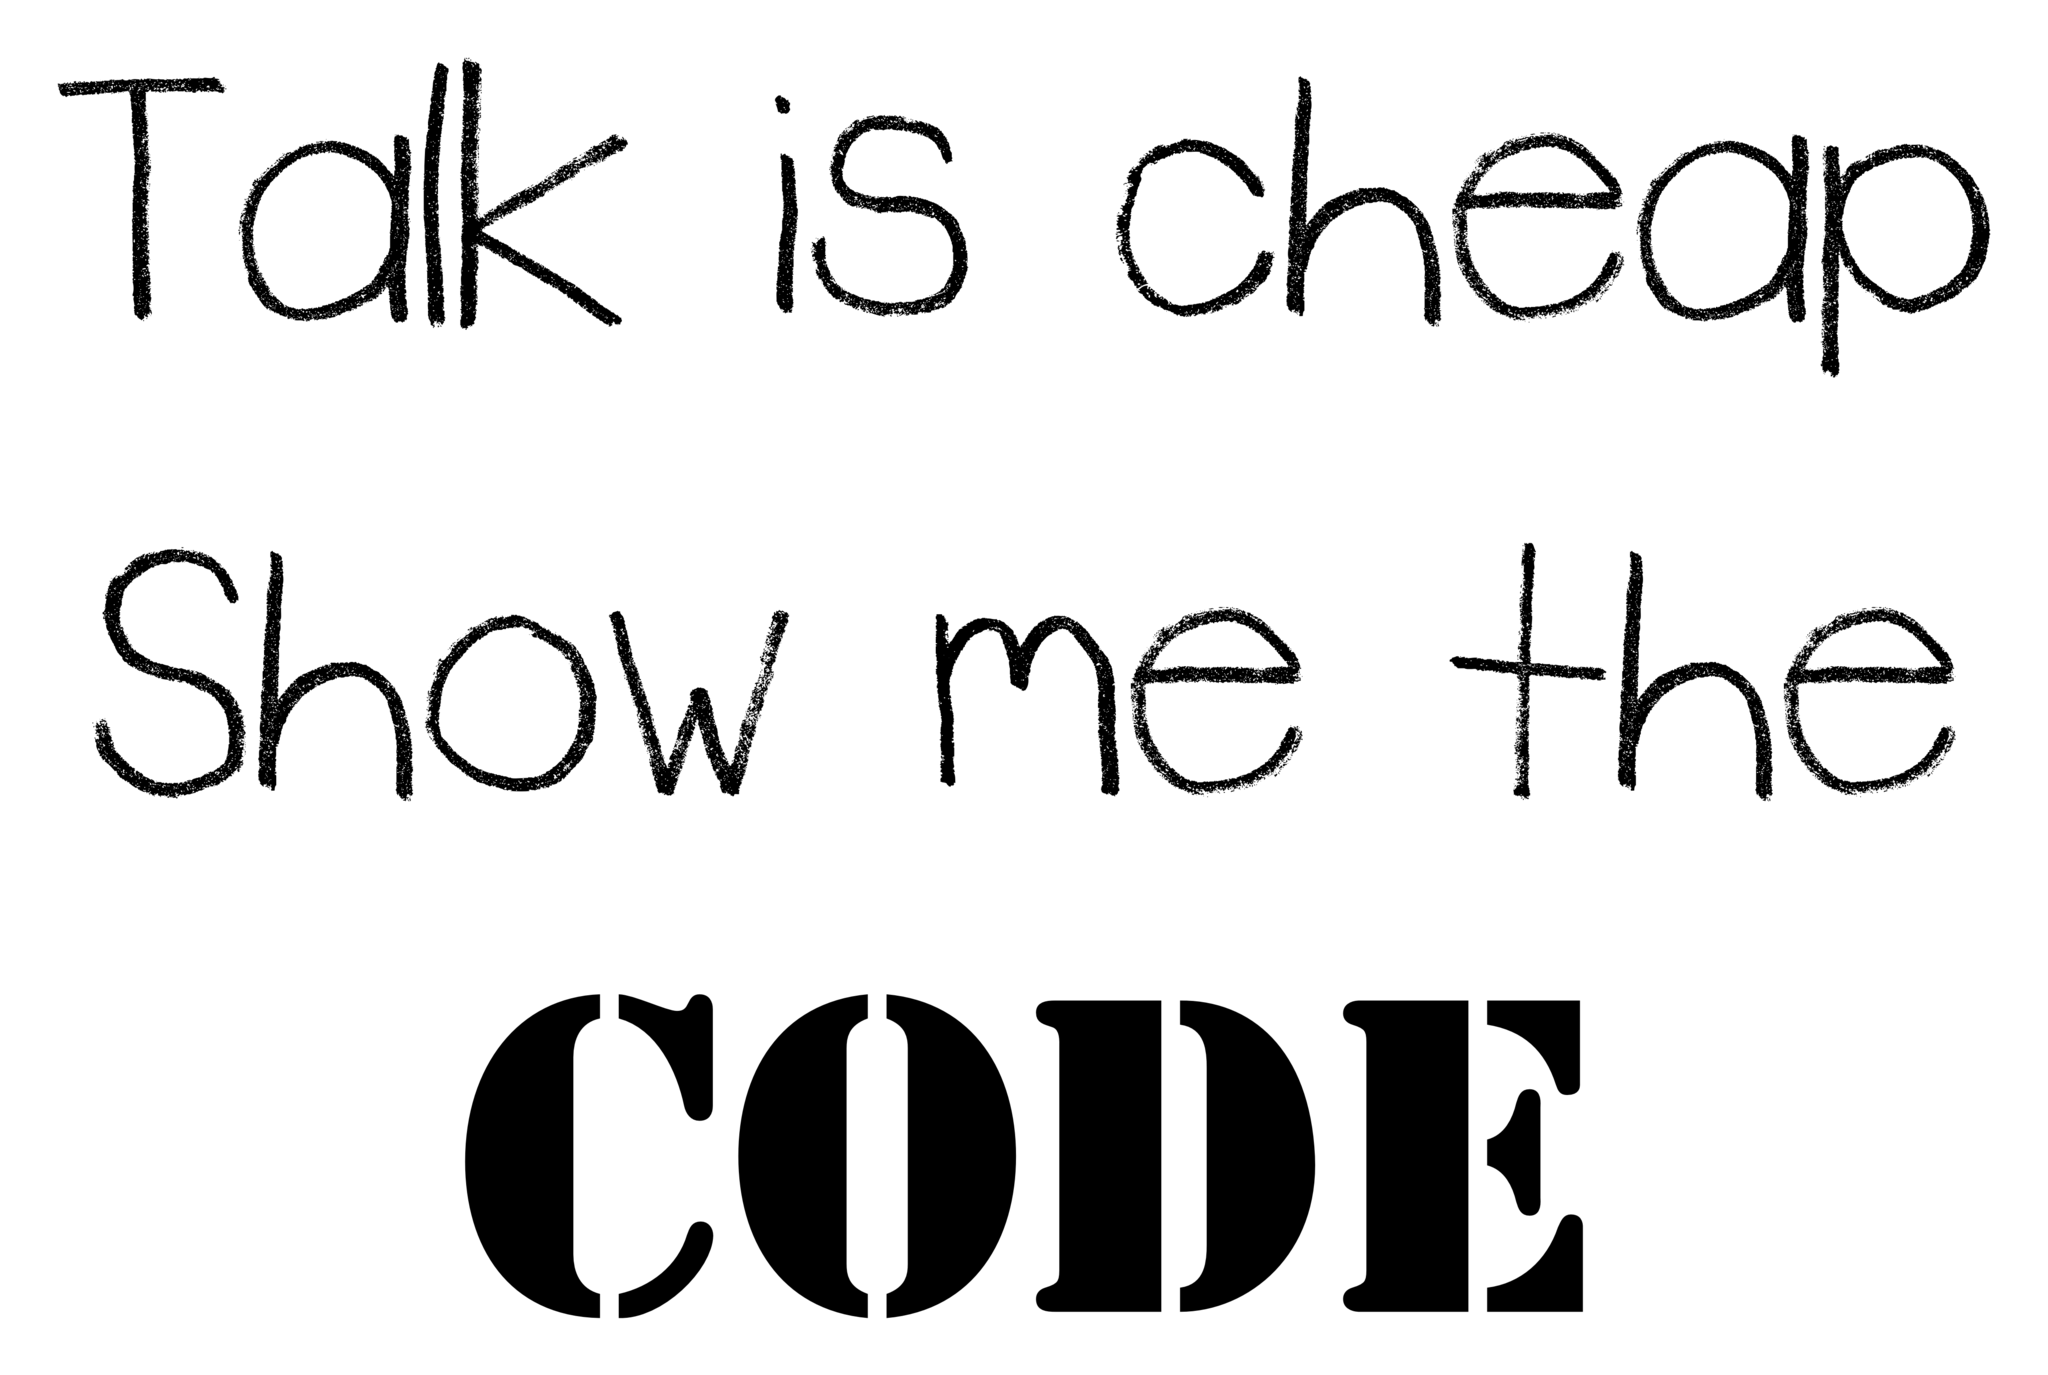
\includegraphics[width=1\linewidth]{img/torvalds.png}
			\end{figure}
		\end{flushright}	
		
	\end{columns}
\end{frame}


%------------------------------------------------
\begin{frame}
	\begin{flushleft}
	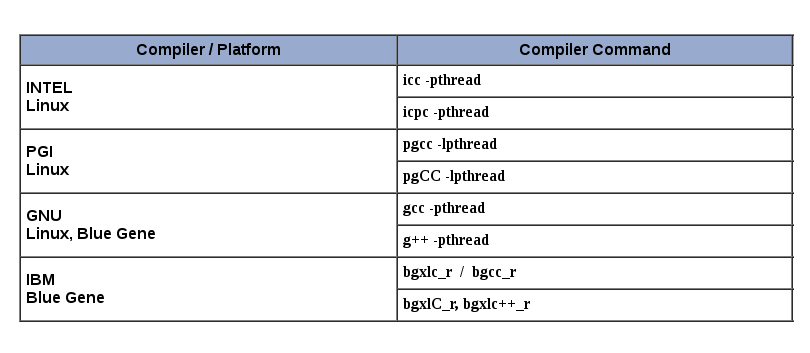
\includegraphics[width=1.1\linewidth]{img/compiling.png}
	\end{flushleft}
\end{frame}

%------------------------------------------------
\begin{frame}

	\begin{columns}
		\column{0.5\textwidth}
			\begin{figure}
				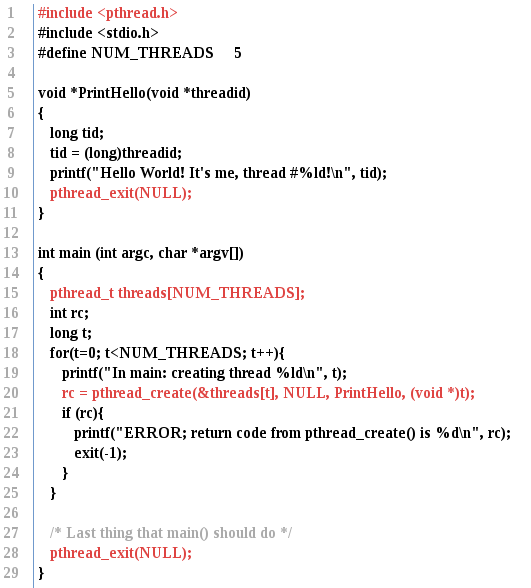
\includegraphics[width=1.2\linewidth]{img/code-thread.png}
			\end{figure}
		

		\column{0.5\textwidth}
		\begin{block}{Saída}
		\footnotesize
			\texttt{In main: creating thread 0\\
				In main: creating thread 1\\
				Hello World! It's me, thread \#0!\\
				In main: creating thread 2\\
				Hello World! It's me, thread \#1!\\
				Hello World! It's me, thread \#2!\\
				In main: creating thread 3\\
				In main: creating thread 4\\
				Hello World! It's me, thread \#4!\\
				Hello World! It's me, thread \#3!
			}
			
		\end{block}
		
	\end{columns}
	
\end{frame}
%------------------------------------------------
\begin{frame}
	\begin{columns}
		\column{0.4\textwidth}
			\begin{figure}
				
\includegraphics[width=.8\linewidth]{img/taserto.png}
				\caption{Vlw Brunão ta Serto, maIs I daew? R: RLX!}
			\end{figure}
		

		\column{0.6\textwidth}
		\begin{block}{Como uso thread com sockets?}
			\begin{itemize}
				\item Relembrando, nosso OJBETIVO ERA:
					\begin{itemize}
						\item Receber várias conexões simultaneas (~)
						\item Saber Threads (\checkmark)
					\end{itemize}
			\end{itemize}
		\end{block}
		
	\end{columns}
\end{frame}

%------------------------------------------------
\section{Usando SELECT}
\begin{frame} \frametitle{Segunda parte}
	\begin{block}{Objetivos}
		\begin{itemize}
			\item Ao final dessa aula você será capaz de:
			\begin{itemize}
				\item Entender o uso de threads
				\item Entender o uso do \textit{Select}
			\end{itemize}
			\item Criar um programa \textbf{SERVIDOR} que aceita conexão de vários clientes
			\begin{itemize}
				\item Usando \textit{Threads}
				\item Usando \textcolor<2->{red}{\textit{Select}}
			\end{itemize}
		\end{itemize}
		\begin{itemize}
			\item<2-> Vamos criar um \textbf{SERVIDOR} que faz uso do SELECT para gerenciar múltiplas conexões
		\end{itemize}
	\end{block}
\end{frame}

%------------------------------------------------
\begin{frame}
	\begin{block}{Scokets - Nomenclatura}
		\begin{itemize}
			\item<1-> Existe uma nomenclatura para cada um dos "lados" da comunicação
			\item<2-> Servidor
				\begin{itemize}
					\item Espera por conexões de entrada
					\item Fornece certos tipos de serviços para a outra parte
				\end{itemize}
			\item<3-> Cliente
				\begin{itemize}
					\item Solicita uma conexão ao servidor
					\item Faz requisições de serviços
				\end{itemize}
			
			\item<4-> Não é o computador quem decide quem é cliente ou quem é servidor, mas sim a forma como o programa usa os sockets.
		\end{itemize}
	\end{block}
\end{frame}
%------------------------------------------------
\begin{frame}
	\begin{columns}
		\column{0.4\textwidth}
			\begin{figure}
				
\includegraphics[width=.8\linewidth]{img/taserto.png}
				\caption{Vlw Brunão ta Serto, maIs I daew? R: RLX!}
			\end{figure}
		

		\column{0.6\textwidth}
		\begin{block}{Como uso thread com sockets?}
			\begin{itemize}
				\item Relembrando, nosso OJBETIVO ERA:
					\begin{itemize}
						\item Receber várias conexões simultaneas (~)
						\item Saber Threads (\checkmark)
					\end{itemize}
			\end{itemize}
		\end{block}
		
	\end{columns}
\end{frame}


%------------------------------------------------

\begin{frame}
	\begin{figure}
		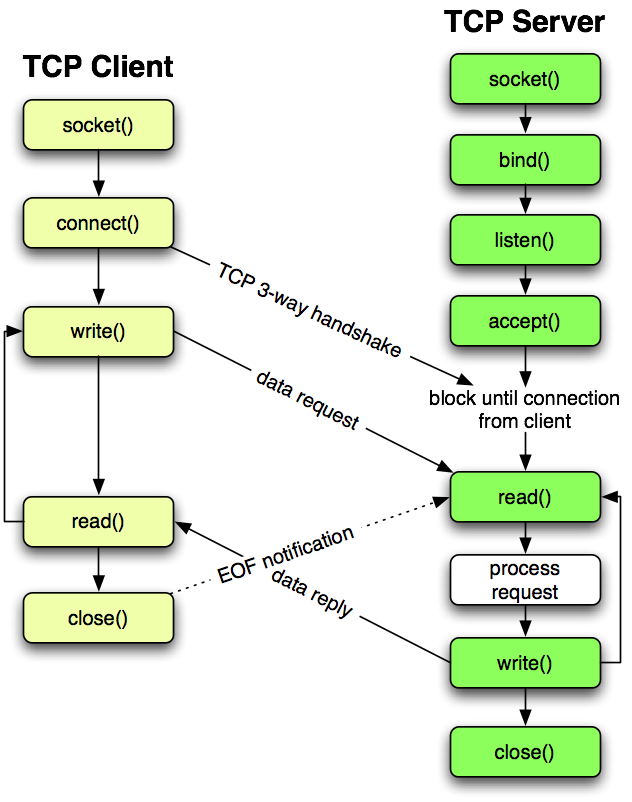
\includegraphics[width=.55\linewidth]{img/tcplab}
	\end{figure}	
\end{frame}

%------------------------------------------------

\begin{frame}
	
	
	\begin{overlayarea}{\textwidth}{10em}
		
		\only<1> {
		\begin{block}{Scokets - Tipos}
			\begin{itemize}
				\item Stream Sockets - SOCK\_STREAM
				\begin{itemize}
					\item Usa o protocolo TCP/IP \footnote{The Transmission Control Protocol RFC 2001\cite{stevens1997tcp}. Internet Protocol address.}
					\item Mantém uma conexão confiável
					\item Os dados vão em ordem
					\item Livre de erros
				\end{itemize}
			\end{itemize}
		\end{block}
		}

		\only<2->{
		\begin{block}{Scokets - Tipos}
			\begin{itemize}
				 \item Datagram Sockets - SOCK\_DGRAM
				 \begin{itemize}
				 	\item Usa o protocolo UDP/IP \footnote{User Datagram Protocol RFC 768\cite{postel1980user}.}
					\item \textbf{Não} mantém uma conexão confiável
					\item \textbf{Não} garante a chegada em ordem dos dados
				\end{itemize}
			\end{itemize}
		\end{block}
		}
	
		\only<3>{
			\begin{figure}
			
\includegraphics[width=1\linewidth]{img/dataencap}
			\end{figure}
		}
	\end{overlayarea}
		
\end{frame}
%------------------------------------------------
\begin{frame}
\begin{columns}
	\begin{column}{4cm}
		\begin{block}{Scokets - Porta}
			\begin{itemize}
				\item<1-> Como saber qual aplicação devo enviar os dados?
				\item<2-> Cada aplicação vai ter uma porta associada
				\begin{itemize}
					\item Comando: less /etc/services
					\item netstat -antp
				\end{itemize}
			\end{itemize}
		\end{block}
	\end{column}
	
	\begin{column}{7cm}
		\begin{figure}
			\includegraphics<1>[width=1\linewidth]{img/net_soc2}
		\end{figure}	
		
		\begin{figure}
		\includegraphics<2>[width=1\linewidth]{img/sockets01}
		\end{figure}
	\end{column}
\end{columns}

\end{frame}
%------------------------------------------------

\begin{frame}
	\begin{figure}
		\includegraphics<1>[width=1\linewidth]{img/port}
	\end{figure}
\end{frame}

%------------------------------------------------
\section{Programação} % Sections can be created in order to organize your presentation into discrete blocks, all sections and subsections are automatically printed in the table of contents as an overview of the talk
%------------------------------------------------
\subsection{Cliente e Servidor} % A subsection can be created just before a set of slides with a common theme to further break down your presentation into chunks
%------------------------------------------------

\begin{frame}\frametitle{Cliente e Servidor}
	\begin{example}{Servidor.c}
		\begin{itemize}
			\item<1-> Veja o código Servidor.c \cite{bruno}
			\item<2-> Comando: nc $<$endereço$>$ $<$porta$>$
			\begin{itemize}
				\item Comando: nc localhost 5050
			\end{itemize}
		\end{itemize}
	\end{example}
	
	\begin{example}<3->{Cliente.c}
		\begin{itemize}
			\item<3-> Veja o código Cliente.c \cite{bruno}
			\item<4-> Execute uma instância do servidor e uma do cliente
		\end{itemize}
	\end{example}
\end{frame}
%------------------------------------------------

%------------------------------------------------

\begin{frame}
	\Fontvi
	\nocite{*}
	\bibliographystyle{plain}
	\bibliography{refs}
\end{frame}
%------------------------------------------------
\section{Extra} % A subsection can be created just before a set of slides with a common theme to further break down your presentation into chunks
%------------------------------------------------

\begin{frame}\frametitle{Extras}
	\begin{example}{ShowIP.c}
		\begin{itemize}
			\item<1-> Veja o código ShowIP.c \cite{bruno}
			\item<2-> Comando: ping $<$endereço$>$
		\end{itemize}
	\end{example}
	
	\begin{example}<3->{client\_beej.c e server\_beej.c}
		\begin{itemize}
			\item<3-> Versão com mais detalhes
			\item<3-> Execute uma instância do servidor e uma do cliente
		\end{itemize}
	\end{example}
\end{frame}

%%------------------------------------------------
%\begin{frame}
%\begin{tiny}
%	\begin{figure}
%		\centering
%        \begin{subfigure}[b]{0.3\textwidth}
%                \includegraphics[width=\textwidth]{img/Degree}
%                \caption{Degree}
%                \label{fig:Degree}
%        \end{subfigure}%
%        \qquad %add desired spacing between images, e. g. ~, \quad, \qquad etc.
%          %(or a blank line to force the subfigure onto a new line)
%        \begin{subfigure}[b]{0.3\textwidth}
%                \includegraphics[width=\textwidth]{img/Closeness}
%                \caption{Closeness}
%                \label{fig:Closeness}
%        \end{subfigure}
%        \qquad %add desired spacing between images, e. g. ~, \quad, \qquad etc.
%          %(or a blank line to force the subfigure onto a new line)
%        \begin{subfigure}[b]{0.3\textwidth}
%                \includegraphics[width=\textwidth]{img/Betweenness}
%                \caption{Betweenness}
%                \label{fig:Betweenness}
%        \end{subfigure}
%        \caption{Centralidade}\label{fig:animals}
%	\end{figure}
%\end{tiny}
%\end{frame}
%
%%------------------------------------------------
%
%\begin{frame}[fragile] \frametitle{Entendendo os grafos - \textit{Betweenness}}
%\begin{scriptsize}
%
%	\begin{block}{Betweenness - O que é?}
%		
%		\begin{itemize}
%			\item Betweenness é uma medida de de centralidade de um vértice em um grafo
%			\item Quantifica o número de vezes que um nó atua como 'ponte' no \textit{menor caminho} entre quais quer dois outros nós do grafo
%			\item Vértices que tem uma alta probabilidade de ser 'ponte' possuem alto valor de betweenness
%		\end{itemize}
%		%Betweenness is a centrality measure of a vertex within a graph (there is also edge betweenness, which is not discussed here). Betweenness centrality quantifies the number of times a node acts as a bridge along the shortest path between two other nodes. It was introduced as a measure for quantifying the control of a human on the communication between other humans in a social network by Linton Freeman.[12] In his conception, vertices that have a high probability to occur on a randomly chosen shortest path between two randomly chosen vertices have a high betweenness.
%	\end{block}
%
%	\begin{example}
%		Betweenness - Vou fazer o que com esse 'trem'?
%		\begin{itemize}
%			\item Foi introduzida para quantificar o controle que um nó possui entre a comunicação de quais quer outros nós
%			\item Numa interação humana, se um indivíduo age como interlocutor entre duas pessoas, aquele será um elemento com alta centralidade
%		\end{itemize}
%	\end{example}
%	
%	
%\end{scriptsize}
%\end{frame}
%
%%------------------------------------------------
%
%\begin{frame}[fragile] \frametitle{Entendendo os grafos - \textit{Betweenness}}
%\begin{scriptsize}
%\begin{columns}[c] % The "c" option specifies centered vertical alignment while the "t" option is used for top vertical alignment
%	\column{.75\textwidth} % Left column and width
%	\begin{block}{Betweenness - Como calcular?}
%		\begin{itemize}
%			\item Betweenness de um vértice $v$ num grafo $G:=(V,E)$, com $V$ vértices é computado como segue:			
%				\begin{enumerate}
%					\begin{scriptsize}
%					\item Para cada par de vértices $(s,t)$, calcule o menor caminho entre eles.
%					\item Para cada par de vértices $(s,t)$, determine a fração do menor caminho que passa pelo vértice em questão (neste caso $v$).
%					\item Some o item anterior sobre todos os pares de vértices $(s,t)$.
%					\end{scriptsize}	
%				\end{enumerate}
%			
%			\item Mais formalmente
%				\begin{itemize}
%					\item $C_B(v)=\sum _{s\neq v \neq t \in V} \frac{\sigma _{st} (v)}{\sigma _{st}}$
%				\end{itemize}
%			
%			\item Complexidade
%				\begin{itemize}
%					\begin{small}
%				
%					\item $\Theta(V^3)$ com \textit{Floyd–Warshall algorithm}
%					\item $O(V^2 log V + VE)$ com \textit{Johnson's algorithm} em grafos esparsos.
%					
%					\end{small}
%				\end{itemize}
%		\end{itemize} 
%	\end{block}
%	
%	\column{.20\textwidth} % Right column and width
%	\begin{figure}
%		\includegraphics[width=1.3\linewidth]{img/Betweenness}
%	\end{figure}	
%\end{columns}
%\end{scriptsize}	
%\end{frame}
%
%
%%------------------------------------------------
%\subsection{Estratégias de roteamento} % A subsection can be created just before a set of slides with a common theme to further break down your presentation into chunks
%
%%------------------------------------------------
%\begin{frame}
%	\frametitle{Estratégias de roteamento}
%	\begin{itemize}
%		\item Protocolos de roteamento
%			\begin{itemize}
%				\item Especificam como os nós em uma rede se comunicam uns com os outros
%				\item Criam uma tabela de rotas (destino $\Rightarrow$ porta)
%				\item As tabelas podem ser alteradas devido a congestionamento ou quedas de links
%				
%				\item Os nós criam árvores geradoras para cada nó de destino na rede
%			\end{itemize}
%		
%		\item Estratégias para protocolos
%			\begin{itemize}
%				\item Manter o menor caminho para os destinos
%				\item Balancear carga de tráfego
%			\end{itemize}
%	\end{itemize}
%	
%	%A maioria dos protocolos de roteamento criam uma tabela de rotas que atribuem para um dado endereço de destino de um pacote uma porta de saída. Ocasionalmente essa tabela é alterada devido a falhas de links ou congestionamentos em determinada rota. Durante o período em que a tabela não é alterada os nós criam arvores geradoras para cada nó de destino na rede. Alguns algoritmos mantém o menor caminho para os destinos, outros balanceiam a carga de trafego encaminhando parte da carga por rotas que não necessariamente são as de menores comprimentos.
%\end{frame}
%%------------------------------------------------
%
%\begin{frame}
%	\frametitle{Estratégias de roteamento}
%	\begin{itemize}
%		\item Shortest Path Betweenness-Centrality (SPBC)
%			\begin{itemize}
%				\item Somente os menores caminhos são utilizados para transferir fluxo na rede\begin{tiny}\footnote{Para fins comercial, fatores como balanceamento de carga, tolerância a falhas e acordos de nível de serviço deve ser considerada. Infelizmente, esses fatores pode levar a fluxos de tráfego que não são roteados por caminhos mais curtos para o alvo}\end{tiny}
%			\end{itemize}
%		\item Traffic Load Centrality (TLC)
%			\begin{itemize}
%				\item Somente os menores caminhos são utilizados para transferir fluxo na rede
%				\item Considera a carga nos links
%			\end{itemize}
%	\end{itemize}
%\end{frame}
%%------------------------------------------------
%\begin{frame}
%	\frametitle{Estratégias de roteamento}
%	\begin{itemize}
%		\item Flow Betweenness-Centrality (FBC)
%			\begin{itemize}
%				\item Considera \textcolor{red}{igualmente} rotas de todos os comprimentos
%				\item Obriga que as rotas percorram caminhos simples\footnote{Rotas que não contém ciclos.}
%			\end{itemize}
%		\item Random Walk Betweenness-Centrality (RWBC)
%			\begin{itemize}
%				\item Assume que os menores caminhos são mais utilizados que os maiores.
%				\item Considera que caminhos \textcolor{red}{podem conter ciclos}\footnote{Não é o caso da maioria das comunicações em rede.}
%			\end{itemize}
%	\end{itemize}
%\end{frame}
%%------------------------------------------------
%
%\begin{frame}
%	\frametitle{Estratégias de roteamento}
%\begin{tiny}
%	\begin{block}{SPBC}
%		Os nos encaminham pacotes para um de seus vizinhos que estão mais próximos do destino. A probabilidade de um nó $u$ encaminha para $v$ um pacote destinado a $t$ é igual a fração dos menores de $u$ para $t$ que passa através de $v$.
%	\end{block}
%	%SPBC:  os nos encaminham pacotes para um de seus vizinhos o qual está mais próximo do destino.  A probabilidade de um nó u encaminha para v um pacote destinado a t é igual a fração dos shortest path de u para t que passa através de v (EQ NO PAPER).
%	
%	\begin{block}{TLC}
%		Os nós encaminham pacotes para um de seus vizinhos que estão mais próximos do destino com probabilidade igual.
%	\end{block}
%%	TCL: os nodos encaminham pacotes para um de seus vizinhos que estão mais próximos do destino com probabilidade igual, neste caso R(...) é igual a 1 dividido pelo numero de vizinhos v mais próximos do destino t.
%	\begin{block}{FBC}
%	Para cada par $(s,t)$ de nós são encaminhados pacotes de $s$ a seus vizinhos para produzir o fluxo maximal entre $s$ e $t$. A probabilidade de $u$ encaminha para $v$ um pacote destinado a $t$ é proporcional a porção de st-fluxo levado pelo link $(u,v)$.
%	\end{block}
%	%FBC: para cada par s, t de nós são encaminhados pacotes de s a um de seus vizinhos para produzir o fluxo maximal entre s e t. A probabilidade de u encaminha para v um pacote destinado a t é proporcional a porção de st-fluxo levado pelo link (u, v): (EQ NO PAPER).
% 
%	\begin{figure}
%		\includegraphics[width=0.8\linewidth]{img/algoritmos}
%	\end{figure}
%\end{tiny}	
%\end{frame}
%%------------------------------------------------
%\begin{frame}
%	\frametitle{Estratégias de roteamento}
%	\begin{itemize}
%		\item \textbf{Routing Betweenness Centrality (RBC) \cite{p1}}
%			\begin{itemize}
%				\item Arbitrário esquema de roteamento \textcolor{red}{sem loop}
%				\item Decisões de roteamento são flexíveis
%					\begin{itemize}
%						\item Fonte e Destino
%						\item Destino
%					\end{itemize}
%				\item SPBC, TCL e FBC são casos particulares do RBC
%			\end{itemize}
%	\end{itemize}
%\end{frame}
%
%
%%------------------------------------------------
%\section{Routing Betweenness Centrality} % A subsection can be created just before a set of slides with a common theme to further break down your presentation into chunks
%%------------------------------------------------
%\begin{frame}\frametitle{Routing Betweenness Centrality - RBC}
%	\begin{itemize}
%		\item Será apresentado algoritmos para:
%		\begin{itemize}
%			\item Calcular o RBC para cada vértice
%			\item Calcular o RBC para um grupo de vértices, desta forma é possível mostrar o potencial de forma colaborativa para controlar e monitorar o fluxo de dados na rede.
%				\begin{itemize}
%					\item Conjuntiva – o grupo é uma sequência de vértices controlando o tráfego e o fluxo deve passar por todos eles de forma ordenada
%					\item Disjuntiva – o grupo de vértices controlando o trafego de modo que ao menos um vértice do grupo processa o tráfego
%				\end{itemize}
%		\end{itemize}
%	\end{itemize}
%\end{frame}
%
%%------------------------------------------------
%\subsection{Para cada nó} % A subsection can be created just before a set of slides with a common theme to further break down your presentation into chunks
%%------------------------------------------------
%\begin{frame} \frametitle{RBC}
%\begin{scriptsize}
%	\begin{block}{RBC - para cada nó}
%		\begin{itemize}
%			\item Complexidade\footnote{$n$ é número de nos na rede e $m$ o maximal número de aresta na árvore de roteamento}
%				\begin{itemize}
%					\item Para fonte e destino $O(n^2 m)$
%					\item Somente destino $O(nm)$
%					%n – number of nodes in the network; m – maximal number of edges in routing trees (or a routing directed acyclic graphs (DAG) for multi-path routing schemes); k – number of nodes in a sequence or a set.
%
%				\end{itemize}
%		\end{itemize}
%	\end{block}
%	\centering
%	\begin{figure}     
%        \begin{subfigure}[b]{0.4\textwidth}
%                \includegraphics[width=\textwidth]{img/single}
%                \caption{Fonte e destino}
%                \label{fig:gull}
%        \end{subfigure}%
%        \qquad %add desired spacing between images, e. g. ~, \quad, \qquad etc.
%          %(or a blank line to force the subfigure onto a new line)
%        \begin{subfigure}[b]{0.4\textwidth}
%                \includegraphics[width=\textwidth]{img/singleOblivious}
%                \caption{Destino óbvio}
%                \label{fig:tiger}
%        \end{subfigure}
%    \end{figure}
%\end{scriptsize}	
%\end{frame}
%%------------------------------------------------
%\subsection{Para sequência} % A subsection can be created just before a set of slides with a common theme to further break down your presentation into chunks
%%------------------------------------------------
%\begin{frame} \frametitle{RBC}
%\begin{scriptsize}
%	\begin{block}{RBC - para um grupo em sequência}
%		\begin{itemize}
%			\item Complexidade\footnote{$n$ é número de nos na rede e $m$ o maximal número de aresta na árvore de roteamento}
%				\begin{itemize}
%					\item Para fonte e destino $O(n^2 m)$
%					\item Somente destino $O(nm)$
%					%n – number of nodes in the network; m – maximal number of edges in routing trees (or a routing directed acyclic graphs (DAG) for multi-path routing schemes); k – number of nodes in a sequence or a set.
%
%				\end{itemize}
%		\end{itemize}
%	\end{block}
%	
%	\centering
%	\begin{figure}     
%        \begin{subfigure}[b]{0.4\textwidth}
%                \includegraphics[width=\textwidth]{img/sequence}
%                \caption{Fonte e destino}
%                \label{fig:gull}
%        \end{subfigure}%
%        \qquad %add desired spacing between images, e. g. ~, \quad, \qquad etc.
%          %(or a blank line to force the subfigure onto a new line)
%        \begin{subfigure}[b]{0.4\textwidth}
%                \includegraphics[width=\textwidth]{img/sequenceOblivious}
%                \caption{Destino óbvio}
%                \label{fig:tiger}
%        \end{subfigure}
%    \end{figure}
%\end{scriptsize}	
%\end{frame}
%
%%------------------------------------------------
%\subsection{Para conjunto} % A subsection can be created just before a set of slides with a common theme to further break down your presentation into chunks
%%------------------------------------------------
%\begin{frame} \frametitle{RBC}
%\begin{scriptsize}
%	\begin{block}{RBC - para um grupo}
%		\begin{itemize}
%			\item Complexidade\footnote{$n$ é número de nos na rede e $m$ o maximal número de aresta na árvore de roteamento}
%				\begin{itemize}
%					\item Para fonte e destino $O(n^2 m)$
%					\item Somente destino $O(nm)$
%					%n – number of nodes in the network; m – maximal number of edges in routing trees (or a routing directed acyclic graphs (DAG) for multi-path routing schemes); k – number of nodes in a sequence or a set.
%
%				\end{itemize}
%		\end{itemize}
%	\end{block}
%	
%	\centering
%	\begin{figure}     
%        \begin{subfigure}[b]{0.4\textwidth}
%                \includegraphics[width=\textwidth]{img/set}
%                \caption{Fonte e destino}
%                \label{fig:gull}
%        \end{subfigure}%
%        \qquad %add desired spacing between images, e. g. ~, \quad, \qquad etc.
%          %(or a blank line to force the subfigure onto a new line)
%        \begin{subfigure}[b]{0.4\textwidth}
%                \includegraphics[width=\textwidth]{img/setOblivious}
%                \caption{Destino óbvio}
%                \label{fig:tiger}
%        \end{subfigure}
%    \end{figure}
%\end{scriptsize}	
%\end{frame}
%
%%------------------------------------------------
%\section{Sink Betweenness}
%%------------------------------------------------
%
%%------------------------------------------------
%\begin{frame} \frametitle{Redes de Sensores Sem Fio (RSSF)}
%	\begin{itemize}
%		\item Usualmente existem duas metas nesse tipo de rede
%			\begin{itemize}
%				\item \textit{Data collection}
%				\item \textit{Data dissemination}
%			\end{itemize}
%		\item Aplicações dirigidas a eventos
%			\begin{itemize}
%				\item A rede é mantida em economia de energia
%				\item Quando acontece um evento os nós constroem uma estrutura de roteamento
%			\end{itemize}
%	\end{itemize}
%\end{frame}
%
%%------------------------------------------------
%\subsection{Definição}
%%------------------------------------------------
%\begin{frame} \frametitle{Definição - \textit{Sink Betweenness}}
%	\begin{itemize}
%		\item O que a métrica proporciona?
%			\begin{itemize}
%				\item Capturar os possíveis cenários de RSSF
%					\begin{itemize}
%						\item comunicação se dá dos nós sensores para o \textit{sink} e vice-versa	
%					\end{itemize}
%				\item Quando acontece um evento é possível construir uma árvore de roteamento
%			\end{itemize}
%	\end{itemize}
%	\begin{scriptsize}
%	\begin{block}{Definição}
%		\begin{itemize}
%			\item Dado um grafo $G(V,E)$, onde $V$ são os nós da rede e $E$ são os links entre os nós.
%			\item O \textit{Sink Betweenness}\footnote{\begin{scriptsize}$s$ é o nó \textit{sink}, $\sigma _{ts}$ é o numero de menores caminhos de $t$ para o sink e $\sigma _{is}$ é o número de menores caminhos de $i$ para o \textit{sink}.\end{scriptsize}} \footnote{\begin{scriptsize}$SP_{i\rightarrow s}$ é o conjunto de todos os menores caminhos de um nó $i$ para o \textit{sink}.\end{scriptsize}} de um nó $t$ é:
%				\begin{itemize}
%					\item $Sbet_t = \sum _{i \in \psi _t} \frac{\sigma _{ts}}{\sigma _{is}}$ 
%					\item $\psi _t = \{i \in V | t \in SP_{i\rightarrow s}\}$
%				\end{itemize}
%		\end{itemize}
%		
%	\end{block}
%	\end{scriptsize}
%\end{frame}
%%------------------------------------------------
%\subsection{Exemplo}
%%------------------------------------------------
%\begin{frame} \frametitle{Exemplo \textit{Sink Betweenness}}
%	\begin{figure}
%		\includegraphics[width=0.8\linewidth]{img/Sbet}
%		\\
%		\cite{p3}
%	\end{figure}
%\end{frame}
%
%%------------------------------------------------
%\section{ETX}
%%------------------------------------------------
%\begin{frame} \frametitle{Expected transmission count (ETX)}
%	\begin{block}{ETX o que é?}
%		\begin{itemize}
%			\item É uma métrica que encontrar caminhos com alto \textit{throughput} em redes sem fio
%			\item ETX considera
%				\begin{itemize}
%					\item Taxas de perdas dos links
%					\item Assimetria entre cada direção dos links
%					\item Interferência nos sucessivos links do caminho
%				\end{itemize}
%		\end{itemize}
%	\end{block}
%%	\begin{block}{Definição}
%%		O ETX de um link é o número previsto de transmissões necessárias para enviar um pacote ao longo desse link, incluindo retransmissões.\\
%%		O ETX de uma rota é a soma do ETX de cada link na rota.
%%	\end{block}
%\end{frame}
%%------------------------------------------------
%\subsection{Definição}
%%------------------------------------------------
%\begin{frame} \frametitle{Expected transmission count (ETX)}
%	\begin{block}{Definição}
%		\begin{itemize}
%			\item O ETX de um link é o número previsto de transmissões necessárias para enviar um pacote ao longo desse link, incluindo retransmissões
%			\begin{itemize}
%				\item $ETX = \frac{1}{d_f \times d_r}$ \footnote{Onde $d_f$ é a probabilidade de um pacote de dados chegar ao destino com sucesso e $d_r$ é a probabilidade do pacote ACK ser recebido com sucesso.}
%			\end{itemize}
%			\item O ETX de uma rota é a soma do ETX de cada link na rota.
%		\end{itemize}
%	\end{block}
%\end{frame}
%
%%------------------------------------------------
%\subsection{Exemplo}
%%------------------------------------------------
%\begin{frame} \frametitle{Exemplo ETX}
%	\begin{figure}
%		\includegraphics[width=0.68\linewidth]{img/etx}
%		\\
%		\cite{p2}
%	\end{figure}
%\end{frame}
%
%%------------------------------------------------
%\section{Considerações finais}
%%------------------------------------------------
%
%\begin{frame} \frametitle{Considerações finais}
%	\begin{itemize}
%		\item Energia
%		\item Mobilidade
%		\item Atualização da árvore de roteamento
%	\end{itemize}
%\end{frame}
%
%%------------------------------------------------
%
%\begin{frame}
%\frametitle{Referências}
%\footnotesize{
%\begin{thebibliography}{99} % Beamer does not support BibTeX so references must be inserted manually as below
%%\bibitem[Smith, 2012]{p1} John Smith (2012)
%%\newblock Title of the publication
%%\newblock \emph{Journal Name} 12(3), 45 -- 678.
%
%\bibitem[Dolev, 2009]{p1} Dolev, Shlomi and Elovici, Yuval and Puzis, Rami, 2009 (2009)
%\newblock Routing Betweenness Centrality
%
%\bibitem[Douglas, 2003]{p2} Douglas S. J. Couto, Daniel Aguayo, John Bicket, Robert Morris (2003)
%\newblock A high-throughput path metric for multi-hop wireless routing
%%\newblock \emph{JMobile computing and networking - MobiCom}
%
%\bibitem[Oliveira, 2010]{p3} Oliveira, E. M. R., Ramos, H. S., Loureiro, A. a. F. (2010)
%\newblock Centrality-based routing for Wireless Sensor Networks
%
%\end{thebibliography}
%}
%
%\end{frame}


%%------------------------------------------------
%\begin{frame}
%\frametitle{Bullet Points}
%\begin{itemize}
%\item Lorem ipsum dolor sit amet, consectetur adipiscing elit
%\item Aliquam blandit faucibus nisi, sit amet dapibus enim tempus eu
%\item Nulla commodo, erat quis gravida posuere, elit lacus lobortis est, quis porttitor odio mauris at libero
%\item Nam cursus est eget velit posuere pellentesque
%\item Vestibulum faucibus velit a augue condimentum quis convallis nulla gravida
%\end{itemize}
%\end{frame}
%
%%------------------------------------------------
%
%\begin{frame}
%\frametitle{Blocks of Highlighted Text}
%\begin{block}{Block 1}
%Lorem ipsum dolor sit amet, consectetur adipiscing elit. Integer lectus nisl, ultricies in feugiat rutrum, porttitor sit amet augue. Aliquam ut tortor mauris. Sed volutpat ante purus, quis accumsan dolor.
%\end{block}
%
%\begin{block}{Block 2}
%Pellentesque sed tellus purus. Class aptent taciti sociosqu ad litora torquent per conubia nostra, per inceptos himenaeos. Vestibulum quis magna at risus dictum tempor eu vitae velit.
%\end{block}
%
%\begin{block}{Block 3}
%Suspendisse tincidunt sagittis gravida. Curabitur condimentum, enim sed venenatis rutrum, ipsum neque consectetur orci, sed blandit justo nisi ac lacus.
%\end{block}
%\end{frame}
%
%%------------------------------------------------
%
%\begin{frame}
%\frametitle{Multiple Columns}
%\begin{columns}[c] % The "c" option specifies centered vertical alignment while the "t" option is used for top vertical alignment
%
%\column{.45\textwidth} % Left column and width
%\textbf{Heading}
%\begin{enumerate}
%\item Statement
%\item Explanation
%\item Example
%\end{enumerate}
%
%\column{.5\textwidth} % Right column and width
%Lorem ipsum dolor sit amet, consectetur adipiscing elit. Integer lectus nisl, ultricies in feugiat rutrum, porttitor sit amet augue. Aliquam ut tortor mauris. Sed volutpat ante purus, quis accumsan dolor.
%
%\end{columns}
%\end{frame}
%
%
%%------------------------------------------------
%\section{Second Section}
%%------------------------------------------------
%
%\begin{frame}
%\frametitle{Table}
%\begin{table}
%\begin{tabular}{l l l}
%\toprule
%\textbf{Treatments} & \textbf{Response 1} & \textbf{Response 2}\\
%\midrule
%Treatment 1 & 0.0003262 & 0.562 \\
%Treatment 2 & 0.0015681 & 0.910 \\
%Treatment 3 & 0.0009271 & 0.296 \\
%\bottomrule
%\end{tabular}
%\caption{Table caption}
%\end{table}
%\end{frame}
%
%%------------------------------------------------
%
%\begin{frame}
%\frametitle{Theorem}
%\begin{theorem}[Mass--energy equivalence]
%$E = mc^2$
%\end{theorem}
%\end{frame}
%
%%------------------------------------------------
%
%\begin{frame}[fragile] % Need to use the fragile option when verbatim is used in the slide
%\frametitle{Verbatim}
%\begin{example}[Theorem Slide Code]
%\begin{verbatim}
%\begin{frame}
%\frametitle{Theorem}
%\begin{theorem}[Mass--energy equivalence]
%$E = mc^2$
%\end{theorem}
%\end{frame}\end{verbatim}
%\end{example}
%\end{frame}
%
%%------------------------------------------------
%
%\begin{frame}
%\frametitle{Figure}
%Uncomment the code on this slide to include your own image from the same directory as the template .TeX file. 
%%\begin{figure}
%%\includegraphics[width=0.8\linewidth]{test}
%%\end{figure}
%\end{frame}
%
%%------------------------------------------------
%
%\begin{frame}[fragile] % Need to use the fragile option when verbatim is used in the slide
%\frametitle{Citation}
%An example of the \verb|\cite| command to cite within the presentation:\\~
%
%This statement requires citation \cite{p1}.
%\end{frame}
%
%%------------------------------------------------
%
%\begin{frame}
%\frametitle{References}
%\footnotesize{
%\begin{thebibliography}{99} % Beamer does not support BibTeX so references must be inserted manually as below
%\bibitem[Smith, 2012]{p1} John Smith (2012)
%\newblock Title of the publication
%\newblock \emph{Journal Name} 12(3), 45 -- 678.
%\end{thebibliography}
%}
%\end{frame}
%
%%------------------------------------------------
%
%\begin{frame}
%\Huge{\centerline{The End}}
%\end{frame}
%
%%----------------------------------------------------------------------------------------

\end{document} 
